\textbf{J}
\begin{figure}[H]
  \centering
  \begin{subfigure}{0.1\textwidth}
    \centering
    \begin{tikzpicture}[scale=0.8]
      \draw(0,0) -- (0,0);
    \end{tikzpicture}
  \end{subfigure}
  \begin{subfigure}{.4\textwidth}
    \centering
    \begin{Karnaugh}{Y}{Z}{ZERO}{SP'}
      \minterms{0, 1, 2, 3, 8, 9, 10, 11}
      \indeterminats{4, 5, 6, 7, 12, 13, 14, 15}
      \implicant{0}{10}{blue}
    \end{Karnaugh}
  \end{subfigure}
  \begin{subfigure}{.4\textwidth}
    \centering
    \begin{Karnaugh}{Y}{Z}{ZERO}{SP'}
      \minterms{6, 7, 8, 9, 10, 11}
      \indeterminats{0, 1, 2, 3, 4, 5, 12, 13, 14, 15}
      \implicant{0}{10}{blue}
    \end{Karnaugh}
  \end{subfigure}

  \begin{subfigure}{0.5\textwidth}
    \centering
    \begin{tikzpicture}[scale=0.8]
      \draw(0,0) -- (0,0);
    \end{tikzpicture}
  \end{subfigure}
  \begin{subfigure}{.4\textwidth}
    \centering
    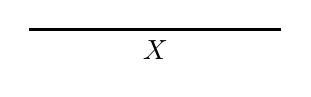
\begin{tikzpicture}[scale=0.8]
      \draw[very thick] (0,0.3) -- node [below]{$X$} ++(4,0);
    \end{tikzpicture}
  \end{subfigure}
  \caption*{$J_Z = 1$.}
\end{figure}

\textbf{K}
\begin{figure}[H]
  \centering
  \begin{subfigure}{0.1\textwidth}
    \centering
    \begin{tikzpicture}[scale=0.8]
      \draw(0,0) -- (0,0);
    \end{tikzpicture}
  \end{subfigure}
  \begin{subfigure}{.4\textwidth}
    \centering
    \begin{Karnaugh}{Y}{Z}{ZERO}{SP'}
      \minterms{0, 1, 2, 3, 8, 9, 10, 11}
      \indeterminats{4, 5, 6, 7, 12, 13, 14, 15}
      \implicantdaltbaix{0}{10}{blue}
      \implicant[3pt]{3}{10}{red}
    \end{Karnaugh}
  \end{subfigure}
  \begin{subfigure}{.4\textwidth}
    \centering
    \begin{Karnaugh}{Y}{Z}{ZERO}{SP'}
      \minterms{0, 1, 2, 3, 14, 15}
      \indeterminats{6, 7, 8, 9, 10, 11}
      \implicantdaltbaix{0}{10}{blue}
      \implicant[3pt]{3}{10}{red}
    \end{Karnaugh}
  \end{subfigure}

  \begin{subfigure}{0.5\textwidth}
    \centering
    \begin{tikzpicture}[scale=0.8]
      \draw(0,0) -- (0,0);
    \end{tikzpicture}
  \end{subfigure}
  \begin{subfigure}{.4\textwidth}
    \centering
    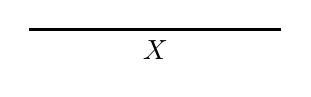
\begin{tikzpicture}[scale=0.8]
      \draw[very thick] (0,0.3) -- node [below]{$X$} ++(4,0);
    \end{tikzpicture}
  \end{subfigure}

  \caption*{$K_Z = \color{blue} \overline{\text{Z}} \color{black} + \color{red} \text{ZERO}$.}
\end{figure}
